  \begin{frame}
    \begin{figure}
      \centering
      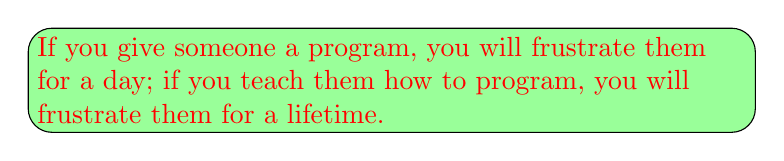
\begin{tikzpicture}
        \node [rectangle,fill=green!40,draw,rounded corners=3mm,text width=9cm,text=red] {
          If you give someone a program, you will frustrate them for a day; 
          if you teach them how to program, you will frustrate them for a lifetime.
        };
      \end{tikzpicture}    
    \end{figure}
  \end{frame}

  \begin{frame}
    \begin{figure}
      \centering
      
\includegraphics[width=2in]{Chapters/Ch01/Fig/DsAlgYan}
      \caption{参考用书}
    \end{figure}
  \end{frame}


\section{数值计算简介}

%%%%%%%%%%%%%%%%%
\begin{frame}\frametitle{\secname} %\fst{现代科学的三大手段}
当今世界科学活动的三种主要方式\\

\begin{itemize}
\item
理论
\item
实验
\item
科学计算
\end{itemize}
\end{frame}
%
%%%%%%%%%%%%%%%%%%
\tikzstyle{decision} = [diamond, draw, fill=blue!20,
text width=4.5em, text badly centered, node distance=3cm, inner sep=0pt]
\tikzstyle{block} = [rectangle, draw, fill=blue!20,
text width=2em, text centered, rounded corners, minimum height=4em]
\tikzstyle{line} = [draw, -latex']
\begin{frame}\ft{\secname}%\fst{解决科学工程问题的步骤}
\begin{figure}
\centering
\begin{tikzpicture}[scale=0.5, node distance = 2.0cm, auto]
  \pause
  \node [block] (problem) {实\\ 际\\ 问\\ 题};

  \pause

  \node [block, right of=problem] (model) {数\\ 学\\ 模\\ 型};
  \path [line] (problem) -- (model);
  \pause

  \node [block, right of=model] (method) {计\\算\\方\\法};
  \path [line] (model) -- (method);
  \pause

  \node [block, right of=method] (prog) {程\\ 序\\ 设\\ 计};
  \path [line] (method) -- (prog);
  \pause

  \node [block, right of=prog] (comp) {上\\ 机\\ 求\\ 解};
  \path [line] (prog) -- (comp);
  \pause

  \draw[decorate, decoration={brace, mirror}, very thick, blue] (0,-3.5) -- (4,-3.5);
  \draw (2,-4.5) node {应用数学};
  \pause

  \draw[decorate, decoration={brace, mirror}, very thick, blue] (8,-3.5) -- (16,-3.5);
  \draw (12,-4.5) node {计算数学};
\end{tikzpicture}
\caption{解决科学工程问题的步骤}
\end{figure}
\end{frame}
%
%%%%%%%%%%%%%%%%%
\begin{frame}\ft{\secname}\fst{研究数值方法的必要性}

\begin{li}
  求解线性方程组
  $$
  Ax = b, \quad A \in \R^{n\times n}, \quad b \in \R^n
  $$
\end{li}
\pause
\begin{dingli}[Crammer法则]
  $$
  A\mbox{非奇异}
  ~~\Longrightarrow~~
  \mbox{此方程组有唯一解,且}
  x_i = \frac{|A_i|}{|A|}, ~~ i = 1, \cd, n.
  $$
\end{dingli}

\pause
该结论非常漂亮,它把线性方程组的求解问题归结为计算$n+1$个$n$阶行列式的计算问题。

\end{frame}
%
%%%%%%%%%%%%%%%%%
\begin{frame}\ft{\secname}\fst{研究数值方法的必要性}

对于行列式的计算
\begin{dingli}[Laplace展开定理]
  $$
  |A| = a_{i1} A_{i1} + a_{i2} A_{i2} +  \cd + a_{in} A_{in}, \quad
  A_{ij}\mbox{为}a_{ij}\mbox{的代数余子式}
  $$      
\end{dingli}

\pause
该方法的运算量大的惊人,以至于完全不能用于实际计算。

\end{frame}
%
%%%%%%%%%%%%%%%%%
\begin{frame}\ft{\secname}

设$k$阶行列式所需乘法运算的次数为$m_k$,则
$$
m_k = k + k m_{k-1},
$$
于是有
$$
\begin{array}{ll}
  &m_n = n + n m_{n-1} \\[0.2cm]
  &= n + n[(n-1) + (n-1) m_{n-2}] \\[0.2cm]
  &= \cd \\[0.2cm]
  &= n + n(n-1) + n(n-1)(n-2) + \cd + n(n-1)\cd 3 \cdot 2\\[0.2cm]
  &> n!
\end{array}
$$

\end{frame}
%
%%%%%%%%%%%%%%%%%
\begin{frame}\ft{\secname}

  故用Crammer法则和Laplace展开定理求解一个$n$阶线性方程组,所需乘法运算的次数就大于
$$
(n+1)n! = (n+1)!.
$$

\end{frame}
%
%%%%%%%%%%%%%%%%%
\begin{frame}\ft{\secname}
在一台百亿次的计算机上求解一个25阶线性方程组,则至少需要
$$
\frac{26!}{10^{10}\times 3600 \times 24 \times 365}
\approx
\frac{4.0329\times 10^{28}}{3.1526\times 10^{17}}
\approx
13\mbox{亿年}
$$
\pause
而用下章介绍的消去法求解,则需要不到一秒钟。
\end{frame}
%
%
%
%%%%%%%%%%%%%%%%%
\begin{frame}\ft{\secname}%\fst{研究对象}
数值分析的研究对象为: 
\begin{itemize}
\item
线性代数\\
\item
曲线拟合\\
\item
数值逼近\\
\item
微积分\\
\item
微分方程\\
\item
积分方程\\
\item
$\cdots$
\end{itemize}
\end{frame}

%%%%%%%%%%%%%%%%%
\begin{frame}\ft{\secname}%\fst{研究任务}
数值分析的研究任务为: 
\begin{itemize}
\item
算法设计 
\item
理论分析
\item[]
\begin{itemize}
\item 算法的收敛性 
\item 稳定性 
\item 误差分析
\end{itemize} 

\item
复杂度分析
\item[]
\begin{itemize}
\item 时间复杂度 
\item 空间复杂度
\end{itemize} 
\end{itemize}

\end{frame}
%
%%%%%%%%%%%%%%%%%
\begin{frame}\ft{\secname}%\fst{特点}
数值分析的特点为: 
\begin{itemize}
\item
既有数学的抽象性与严格性,又有广泛的应用性;
\item
有自身的研究方法和理论系统;
\item
与计算机紧密结合,实用性很强。
\end{itemize}

\end{frame}

\section{数值线性代数}

%%%%%%
\begin{frame}\ft{\secname}%\fst{三大基本问题}
\begin{small}

数值线性代数研究的三大基本问题为:\vspace{0.1in}

\begin{block}{一、求解线性方程组}
给定非奇异矩阵$A\in\R^{n\times n}$和向量$b\in\R^n$,求向量$x\in\R^n$使得
$$
Ax = b.
$$
\end{block}
\end{small}
\end{frame}

\begin{frame}\ft{\secname}
\begin{small}
\begin{block}{二、线性最小二乘问题}
给定矩阵$A\in\R^{m\times n}$和向量$b\in\R^n$,求向量$x\in\R^m$使得
$$
\|Ax - b\|_2 = \min \{\|Ax - b\|_2:~ y \in \R^n \}.
$$
\end{block}
\end{small}
\end{frame}

\begin{frame}\ft{\secname} 
\begin{small}
\begin{block}{三、特征值问题}
给定方阵$A\in\R^{n\times n}$,求其特征值(部分或全部)以及对应的特征向量。
\end{block}
\end{small}
\end{frame}


%%%%%%
\begin{frame}\ft{\secname}%\fst{其他问题}
\begin{small}
数值线性代数所研究的其他问题还有:
\begin{itemize}
\item
约束最小二乘问题
\item
完全最小二乘问题
\item
矩阵方程的求解问题
\item
矩阵函数的计算问题
\item
广义特征值问题
%\item
%非线性特征值问题
\item
特征值反问题
\item
\colorbox{fcolor5}{奇异值分解的计算问题}
\end{itemize}
\end{small}
\end{frame}

\section{逻辑结构和物理结构}

\subsection{逻辑结构}
\begin{frame}
  \documentclass{article}
\usepackage{CJK} 
\usepackage{graphics}
\usepackage{pgf}
\usepackage{tikz}
\usetikzlibrary{calc,shadows}
\usetikzlibrary{decorations.markings,scopes}
\usetikzlibrary{arrows,snakes,backgrounds,shapes}
\usetikzlibrary{decorations.pathmorphing}
\newcommand{\blue}{\textcolor{blue}}
\newcommand{\red}{\textcolor{red}}
\newcommand{\purple}{\textcolor{purple}}


\pgfrealjobname{survey}
\begin{document}
\begin{CJK}{UTF8}{gkai} 
  \beginpgfgraphicnamed{LogicStruct}
  \begin{tikzpicture}[scale=2,cap=round]

    % The graphic
    \node at (0,0)[fill=blue!20,draw,starburst,drop shadow,text width=4.5cm]
    {
      \blue{\large 逻辑结构}: 指数据结构中数据元素之间的相互关系.
    } ;

    \node at (0,-1.6) [text width=2.3cm,decorate,decoration=saw,fill=blue!20,draw,circle]
          {
            \begin{itemize}
            \item 集合结构
            \item 线性结构
            \item 树形结构
            \item 图形结构
            \end{itemize}
          };

  \end{tikzpicture}
  \endpgfgraphicnamed  
\end{CJK}

\end{document}

\end{frame}

\begin{frame}
  \documentclass{article}
\usepackage{CJK} 
\usepackage{graphics}
\usepackage{pgf}
\usepackage{tikz}
\usetikzlibrary{calc,shadows}
\usetikzlibrary{decorations.markings,scopes}
\usetikzlibrary{arrows,snakes,backgrounds,shapes}
\usetikzlibrary{decorations.pathmorphing}
\newcommand{\blue}{\textcolor{blue}}
\newcommand{\red}{\textcolor{red}}
\newcommand{\purple}{\textcolor{purple}}


\pgfrealjobname{survey}
\begin{document}
\begin{CJK}{UTF8}{gkai} 
  \beginpgfgraphicnamed{SetStruct}
  
  \begin{tikzpicture}[scale=2,cap=round]

    % The graphic
    \node at (0,2)[fill=blue!20,draw,starburst,drop shadow,text width=6cm]
    {
      \blue{\large 集合结构}: 其中的元素除了同属于一个集合外,之间没有其他关系.
    } ;
    
    \draw (0,0)circle(1);
    \draw (0.00,0.00)node[]{1}circle(0.15);
    \draw (0.55,0.50)node[]{2}circle(0.15);
    \draw (-.65,-.10)node[]{3}circle(0.15);
    \draw (-.35,0.30)node[]{4}circle(0.15);
    \draw (0.80,0.10)node[]{5}circle(0.15);
    \draw (0.25,-.70)node[]{6}circle(0.15);
    \draw (-.15,0.70)node[]{7}circle(0.15);
    \draw (-.45,-.50)node[]{8}circle(0.15);
    \draw (0.55,-.20)node[]{9}circle(0.15);
  \end{tikzpicture}
  \endpgfgraphicnamed  
\end{CJK}

\end{document}

\end{frame}

\begin{frame}
  \begin{figure}  
  \centering
  \begin{tikzpicture}
    \tikzstyle{state}=[draw,circle]

        % The graphic
    \node at (-.5,2)[left,fill=blue!20,draw,starburst,drop shadow,text=red,text centered]
    (1){
      {线性结构}
    } ;
    \node at (.5,2)[right,fill=blue!20,draw,rectangle,rounded corners=3mm,text=blue,text width=7cm]
    (2){
      其中的数据元素之间是一对一的关系.
    }; 
    \pause    
    \node at (0,0) [state] (1) {1};
    \node[state] (2) [right of=1] {2};
    \node[state] (3) [right of=2] {3};
    \node[state] (4) [right of=3] {4};
    \node[state] (5) [right of=4] {5};
    \node[state] (6) [below of=5] {6};
    \node[state] (7) [below of=6] {7};
    \node[state] (8) [left  of=7] {8};
    \node[state] (9) [left  of=8] {9};
    \path 
    (1) edge (2)
    (2) edge (3)
    (3) edge (4)
    (4) edge (5)
    (5) edge (6)
    (6) edge (7)
    (7) edge (8)
    (8) edge (9);
  \end{tikzpicture}
\end{figure}

\end{frame}

\begin{frame}
  \begin{figure}  
  \centering
  \begin{tikzpicture}[level distance=1.5cm,
    level 1/.style={sibling distance=3cm},
    level 2/.style={sibling distance=1.5cm},
    ]
    \tikzstyle{state}=[draw,circle]
        % The graphic
    \node at (-.5,2)[left,fill=blue!20,draw,starburst,drop shadow,text=red,text centered]
    (1){
      {树形结构}
    } ;
    \node at (0.5,2)[right,fill=blue!20,draw,rectangle,rounded corners=3mm,text=blue,text width=6cm]
    (2){
      其中的数据元素之间是一对多的层次关系.
    };
    \pause
    
    \node[state]{A}
    child {node[state]{B}     
      child {node[state]{E}}
      child {node[state]{F}}
      child {node[state]{G}}
    }
    child {node[state]{C}
      child {node[state]{H}}
    }
    child {node[state]{D}     
      child {node[state]{I}}
      child {node[state]{J}}
    };
    
  \end{tikzpicture}
\end{figure}

\end{frame}

\begin{frame}
  \begin{figure}  
  \centering
  \begin{tikzpicture}[scale=1.5]
    \tikzstyle{state}=[draw,circle]

        % The graphic
    \node at (-.5,1.5)[left,fill=blue!20,draw,starburst,drop shadow,text=red,text centered]
    (1){
      {图形结构}
    } ;
    \node at (0.5,1.5)[right,fill=blue!20,draw,rectangle,rounded corners=3mm,text=blue,text width=6.5cm]
    (2){
      其中的数据元素之间是多对多的关系.
    };
    \pause
    \node at (0,0) [state] (1) {1};
    \node at (-1,-0.5) [state] (2)  {2};
    \node at (1.2,-0.5)[state] (3)  {3};
    \node at (-1.5,-1.5)[state] (4)  {4};
    \node at (0.2,-0.8)[state] (5)  {5};
    \node at (0.8,-2.0)[state] (7)  {7};
    \node at (1.8,-2.5)[state] (6)  {6};
    \node at (-0.5,-1.4)[state] (8)  {8};
    \node at (0.1,-2.8)[state] (9)  {9};
    \path 
    (1) edge (2) edge (3)
    (2) edge (4) edge (8) edge (5)
    (3) edge (5) edge (6)
    (4) edge (8) edge (9)
    (5) edge (7) edge (9)
    (6) edge (9)
    (7) edge (6) edge (9)
    (8) edge (9);
  \end{tikzpicture}
\end{figure}

\end{frame}

\begin{frame}
  在用示意图表示数据的逻辑结构时,请注意: \vspace{0.1in}
  
  \begin{itemize}
  \item 将每一个数据元素看做一个结点,用圆圈表示;\\[0.1in]
  \item 元素之间的逻辑关系用结点之间的连线表示,如果这个关系是有方向的,那么用带箭头的连线表示。
  \end{itemize}
  \pause

  \begin{figure}    
    \centering
    \begin{tikzpicture}
      \node [fill=red!20,starburst,drop shadow,draw,text width=7.5cm,text=blue]{
        逻辑结构是针对具体问题的,是为了解决某个问题。在对问题理解的基础上,选择一个合适的数据结构表示数据元素之间的逻辑关系。      
      };
    \end{tikzpicture}

  \end{figure}

\end{frame}


\subsection{物理结构}

\begin{frame}
  
  \documentclass{article}
\usepackage{CJK} 
\usepackage{graphics}
\usepackage{pgf}
\usepackage{tikz}
\usetikzlibrary{calc,shadows}
\usetikzlibrary{decorations.markings,scopes}
\usetikzlibrary{arrows,snakes,backgrounds,shapes}
\usetikzlibrary{decorations.pathmorphing}
\newcommand{\blue}{\textcolor{blue}}
\newcommand{\red}{\textcolor{red}}
\newcommand{\purple}{\textcolor{purple}}


\pgfrealjobname{survey}
\begin{document}
\begin{CJK}{UTF8}{gkai} 
  \beginpgfgraphicnamed{PhyStruct}
  \begin{tikzpicture}[scale=1.5]
    \tikzstyle{state}=[draw,circle]

        % The graphic
    \node at (0,0)[fill=blue!20,draw,starburst,drop shadow,text width=6.5cm]{
      \blue{\large 物理结构}: 指数据的逻辑结构在计算机中的存储方式.
    } ;

    \node at (-1,-2) [fill=blue!20,draw,ellipse callout, callout relative pointer={(0.,0.7)},text width=5.5cm]{ 
      数据的存储结构应正确反映数据元素之间的逻辑关系。如何存储数据元素之间的逻辑关系,是实现物理结构的重点和难点。
    };

    \node at (2.5,-1.3) [text width=1.5cm,decorate,decoration=saw,fill=blue!20,draw,circle,text=red]{
      顺序存储 链式存储
    };

    
  \end{tikzpicture}
  \endpgfgraphicnamed  
\end{CJK}

\end{document}



  
\end{frame}

\begin{frame}
  
  \documentclass{article}
\usepackage{CJK} 
\usepackage{graphics}
\usepackage{pgf}
\usepackage{tikz}
\usetikzlibrary{calc,shadows}
\usetikzlibrary{decorations.markings,scopes}
\usetikzlibrary{arrows,snakes,backgrounds,shapes}
\usetikzlibrary{decorations.pathmorphing}
\newcommand{\blue}{\textcolor{blue}}
\newcommand{\red}{\textcolor{red}}
\newcommand{\purple}{\textcolor{purple}}


\pgfrealjobname{survey}
\begin{document}
\begin{CJK}{UTF8}{gkai} 
  \beginpgfgraphicnamed{SeqStruct}
  \begin{tikzpicture}[scale=1.5]
    \tikzstyle{state}=[draw,circle]

        % The graphic
    \node at (0,2)[right,fill=blue!20,draw,starburst,drop shadow,text width=6.5cm]{
      \blue{\large 顺序存储结构} \\
      把数据元素存放在连续的存储单元里,其数据间的逻辑关系与物理关系一致。
    } ;

    %% \node at (-1,-2) [fill=blue!20,draw,ellipse callout, callout relative pointer={(0.,0.7)},text width=5.5cm]{ 
    %%   数据的存储结构应正确反映数据元素之间的逻辑关系。如何存储数据元素之间的逻辑关系,是实现物理结构的重点和难点。
    %% };

    %% \node at (2.5,-1.3) [text width=1.5cm,decorate,decoration=saw,fill=blue!20,draw,circle,text=red]{
    %%   顺序存储 链式存储
    %% };
    \def\xx{0.8}
    \draw[very thick] (0,0)--(9*\xx,0);
    \foreach \i in {0,...,9} 
    \draw[very thick] (\i*\xx,0)--(\i*\xx,1*\xx);      
    \foreach \i in {1,...,9} 
    \draw[thick] (\i*\xx-0.5*\xx,0.5*\xx)node[]{\i}circle(0.5*\xx);

    
  \end{tikzpicture}
  \endpgfgraphicnamed  
\end{CJK}

\end{document}



  
\end{frame}

\begin{frame}
  
  \documentclass{article}
\usepackage{CJK} 
\usepackage{graphics}
\usepackage{pgf}
\usepackage{tikz}
\usetikzlibrary{calc,shadows}
\usetikzlibrary{decorations.markings,scopes}
\usetikzlibrary{arrows,snakes,backgrounds,shapes}
\usetikzlibrary{decorations.pathmorphing}
\newcommand{\blue}{\textcolor{blue}}
\newcommand{\red}{\textcolor{red}}
\newcommand{\purple}{\textcolor{purple}}


\pgfrealjobname{survey}
\begin{document}
\begin{CJK}{UTF8}{gkai} 
  \beginpgfgraphicnamed{LinkStruct}
  \begin{tikzpicture}[->,>=stealth,scale=1.5]
    \tikzstyle{state}=[draw,circle]

        % The graphic
    \node at (0,2)[right,fill=blue!20,draw,starburst,drop shadow,text width=6.5cm]{
      \blue{\large 链式存储结构} \\
      把数据元素存放在任意的存储单元里,这组存储单元可以连续,也可以不连续。
    } ;

    \node at (5,-1) [fill=blue!20,draw,ellipse callout, callout relative pointer={(0.,0.7)},text width=4cm]{ 
      数据元素的存储关系并不能反映其逻辑关系,需要用一个指针存放数据元素的地址,这样就可以通过地址找到相关联数据元素的位置。
    };

    
    \node at (0,0)    [state] (1) {1};
    \node at (2.3,-0.3) [state] (2)  {2};
    \node at (2.7,0.1) [state] (9)  {9};
    \node at (1.6,-0.6) [state] (3)  {3};
    \node at (1.0,-1.2) [state] (5)  {5};
    \node at (0.0,-1.8) [state] (8)  {8};
    \node at (1.3,-2.5) [state] (6)  {6};
    \node at (2.4,-2.3) [state] (4)  {4};
    \node at (2.6,-1.0) [state] (7)  {7};
    
    \path (1) edge [bend left] (2)
    (2) edge [bend right] (3)
    (3) edge [bend left] (4)
    (4) edge [bend left] (5)
    (5) edge [bend right] (6)
    (6) edge [bend right] (7)
    (7) edge [bend left] (8)
    (8) edge [bend left] (9)
    ;
    
  \end{tikzpicture}
  \endpgfgraphicnamed  
\end{CJK}

\end{document}



  
\end{frame}

\begin{frame}
  
  \documentclass{article}
\usepackage{CJK} 
\usepackage{graphics}
\usepackage{pgf}
\usepackage{tikz}
\usetikzlibrary{calc,shadows}
\usetikzlibrary{decorations.markings,scopes}
\usetikzlibrary{arrows,snakes,backgrounds,shapes}
\usetikzlibrary{decorations.pathmorphing}
\newcommand{\blue}{\textcolor{blue}}
\newcommand{\red}{\textcolor{red}}
\newcommand{\purple}{\textcolor{purple}}


\pgfrealjobname{survey}
\begin{document}
\begin{CJK}{UTF8}{gkai} 
  \beginpgfgraphicnamed{LogicPhySummary}
  \begin{tikzpicture}
  \node[copy shadow,fill=blue!20,draw=blue,thick,text width=7cm] at (3.5,0) {
    逻辑结构是面向问题的,而物理结构是面向计算机的,我们的目标是将数据及其逻辑关系存储到计算机的内存中。
  };
\end{tikzpicture}
  \endpgfgraphicnamed  
\end{CJK}

\end{document}



  
\end{frame}

\section{选用和设计算法应遵循的原则}

%******
\begin{frame}\ft{原则1:数值稳定} 

\begin{flushleft}
一、选用{数值稳定}的计算公式,控制舍入误差的传播
\end{flushleft}
若算法不稳定,则数值计算的结果就会严重背离数学模型的真实结果。
因此在选择数值计算公式来进行近似计算时,应特别注意选用那些在计算过程中不会导致误差迅速增长的计算公式。
\end{frame}

%******
\begin{frame}\ft{原则1:数值稳定} 
\begin{li}
计算积分
$$
I_n = e^{-1} \int_0^1 x^n e^x \,dx, ~~~ n = 0, 1, 2, \cdots
$$
\end{li}
\pause
$$
\textcolor{acolor2}{
\mbox{(算法1)}~\cd\cd~
\left\{
\begin{array}{l}
I_n = 1 - n I_{n-1}, \\[0.3cm]
I_0 = 1 - e^{-1} \approx 0.6321.
\end{array}
\right.
}
$$
\end{frame}


%%******
\begin{frame}[fragile]\ft{原则1:数值稳定} 
\begin{lstlisting}[language=matlab,title=matlab code,frame=single,backgroundcolor=\color{red!10}]
t0 = 0.6321;
for i = 1:9
    fprintf('%10.5f ', t0);
    if(mod(i, 3)==0)
        fprintf('\n');
    end
t1 = 1 - i * t0;
t0 = t1;  
end
\end{lstlisting}
\end{frame}


%%******
\begin{frame}[fragile]\ft{原则1:数值稳定}  
\begin{lstlisting}[title=running result,frame=single,backgroundcolor=\color{blue!10}]
0.63210    0.36790    0.26420 
0.20740    0.17040    0.14800 
0.11200    0.21600   -0.72800 
\end{lstlisting}

 
\end{frame}


\begin{frame}\ft{原则1:数值稳定}  
由
$$
0 < I_n < e^{-1} \max_{0\le x \le 1} (e^x) \int_0^1 x^n \,dx = \frac1{n+1}
$$
知
$$
I_7 < \frac1{8} = 0.1250,
~~~ I_8 < \frac1{9} \approx 0.1111,
$$
\pause
\begin{block}{原因}
$I_0$本身有不超过$0.5\times10^{-4}$的舍入误差,
此误差在运算中传播、积累很快,传播到$I_7$和$I_8$时,该误差已放大了7与8倍,从而使得$I_7$和$I_8$的结果面目全非。
\end{block}
\end{frame}

%******
\begin{frame}\ft{原则1:数值稳定}


$$
\textcolor{acolor2}{\mbox{(算法2)}~\cd\cd~~ I_{n-1} = \frac1n(1-I_n)}
$$


\pause 
由
$$
I_n > e^{-1} \min_{0\le x \le 1} (e^x) \int_0^1 x^n \,dx = \frac{e^{-1}}{n+1}
$$
知
$$
\frac{e^{-1}}{n+1} < I_n < \frac1{n+1}.
$$

$$
I_7 \approx 0.1124.
$$

 
\end{frame}


%******
\begin{frame}[fragile]\ft{原则1:数值稳定}

\begin{lstlisting}[language=matlab,title=matlab code,frame=single,backgroundcolor=\color{red!10}]
t0 = 0.1124;
for i = 7:-1:0
    fprintf('%10.5f ', t0);
    if(mod(7-i+1, 3)==0)
        fprintf('\n');
    end
t1 = (1 - t0) / i;
t0 = t1;    
end
\end{lstlisting}
\end{frame}


%******
\begin{frame}[fragile]\ft{原则1:数值稳定} 
\begin{lstlisting}[title=running result,frame=single,backgroundcolor=\color{blue!10}]
0.11240    0.12680    0.14553 
0.17089    0.20728    0.26424 
0.36788    0.63212 
\end{lstlisting}

 
\end{frame}
%
%
%*****
\begin{frame}\ft{原则1:数值稳定}

\begin{dingyi}[数值稳定]
在数值计算中,误差不会增长的计算格式称为是\textcolor{acolor5}{数值稳定}的,否则就是不稳定的。
\end{dingyi}
 
\end{frame}
%
%
%******
\begin{frame}\ft{原则2:简化计算步骤} 

\begin{flushleft}
二、尽量简化计算步骤,以便减少运算次数
\end{flushleft}
\pause 
节省计算量,提高计算速度,简化逻辑结构,减少误差积累。

 
\end{frame}


%******
\begin{frame}\ft{原则2:简化计算步骤}

\begin{li}
计算多项式
$$
P_n(x) = a_n x^n + a_{n-1} x^{n-1} + \cdots + a_1 x + a_0
$$
\end{li}


\begin{itemize}
\item
\textcolor{acolor5}{逐项计算}
\item[]
共需
$$
1+2+\cdots+(n-1)+n=\frac12n(n+1)
$$
次乘法和$n$次加法;
\end{itemize}
\end{frame}


%******
\begin{frame}\ft{原则2:简化计算步骤}
\begin{itemize}
\item
\textcolor{acolor5}{秦九韶算法}
$$
\left\{
\begin{array}{ll}
u_0 = a_n, & \\[0.2cm]
u_k = u_{k-1} x + a_{n-k}, & k = 1, 2, \cdots, n.
\end{array}
\right.
$$
\item[]
共需$n$次乘法和$n$次加法。
\end{itemize}
\end{frame}
%
%
%%%%%%%%%%%%%%%%%%%%%%%%%%%%%%%%55
\begin{frame}\ft{原则2:简化计算步骤}
\textcolor{acolor5}{秦九韶}(1208年-1261年),南宋官员、数学家,与\textcolor{acolor5}{李冶、杨辉、朱世杰}并称宋元数学四大家。
\begin{figure}
\begin{tabular}{cc}   
\begin{minipage}{0.35\linewidth}
\centerline{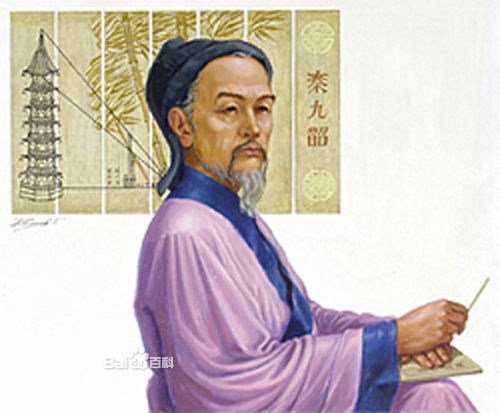
\includegraphics[width=4.0cm]{Chapters/Ch01/figure/qinjiushao.jpg}}
\end{minipage}
\hfill
\begin{minipage}{.6\linewidth}
\begin{itemize}
\item {数学九章}
\item {大衍求一术}
\item[] ~~比Gauss的同余理论早554年
\item  {任意次方程的数值解法}
\item[] ~~比英国人霍纳早提出572年
\item  {三斜求积术}
\item[] ~~海伦公式(公元50年左右)
\item {秦九韶公式}
\item {$\cd$}
\end{itemize}
\end{minipage}
\end{tabular}
\end{figure}
\end{frame}

%******
\begin{frame}\ft{原则3:避免两相近数相减} 
\begin{flushleft}
三、避免两个相近的数相减
\end{flushleft}
\pause 
数值计算中,两个相近的数相减会造成有效数字的严重丢失。
\pause 

\textcolor{acolor3}{处理办法}:
\begin{itemize}
\item
因式分解
\item
分子分母有理化
\item
三角函数恒等式
\item
Taylor展开式
\item
$\cdots$
\end{itemize}
 
\end{frame}
%
%
%
%******
\begin{frame}\ft{原则3:避免两相近数相减} 
\begin{li}
计算(取$4$位有效数字)
$$
\sqrt{x+1} -  \sqrt{x} ~~~~ (x = 1000)
$$
\end{li}
\pause
\begin{itemize}
\item
\textcolor{acolor5}{直接计算}
$$
\sqrt{1001} -  \sqrt{1000} \approx 31.64 - 31.62 = 0.02
$$
只有一个有效数字,损失了三位有效数字;\\[0.2cm]\pause
\item
\textcolor{acolor5}{分子有理化}
$$
\sqrt{x+1} -  \sqrt{x}  = \frac1{\sqrt{x+1} +  \sqrt{x}} \approx 0.01581
$$
没有损失有效数字。
\end{itemize}
\end{frame}

%
%******
\begin{frame}\ft{原则3:避免两相近数相减} 

\begin{li}
计算(取$4$位有效数字)
$$
A = 10^7(1-\cos 2^{\circ}) ~~~~ (\cos 2^{\circ} = 0.9994)
$$
\end{li}

\pause 
\begin{itemize}
\item
\textcolor{acolor5}{直接计算}
$$
A \approx 10^7(1-0.9994)  = 6 \times 10^3
$$
只有一个有效数字\\[0.2cm]\pause
\item
\textcolor{acolor5}{三角恒等式}
$\textcolor{acolor3}{\boxed{
  1 - \cos x = 2 \sin^2 \frac x2 
}}
$
$$
\begin{array}{ll}
A &= 10^7(1-\cos 2^{\circ})  = 2 \times (\sin 1^{\circ})^2 \times 10^7 \\[0.2cm]
&\approx 2 \times 0.01745^2 \times 10^7  \approx 6.09 \times 10^3
\end{array}
$$
三位有效数字
\end{itemize}
\end{frame}
%
%
%******
\begin{frame}\ft{原则4:避免绝对值很小的数做分母}%\fst{}

\begin{flushleft}
四、绝对值太小的数不宜做除数
\end{flushleft}
数值计算中,用绝对值很小的数作除数,会使商的数量级增加,甚至在计算机中造成“溢出”停机,
而且当很小的除数稍有一点误差,会对计算结果影响很大。
\pause 
\begin{li}
$$
\begin{array}{cl}
\ds \frac{3.1416}{0.001} & = 3141.6 \\[0.4cm]
\ds \frac{3.1416}{0.001+0.0001} & = 2856 
\end{array}
$$
\end{li}

\end{frame}



%******
\begin{frame}\ft{原则5:防止大数吃小数} 

\begin{flushleft}
五、合理安排运算次序,防止“大数吃小数”
\end{flushleft}

\begin{li}
计算$a, ~b, ~c$的和,其中$a = 10^{12}, ~b = 10, ~c \approx -a$.
\end{li}
\pause 

\begin{itemize}
\item
$(a+b)+c$
\item[]
~~~~结果接近于0; \pause
\item
$(a+c)+b$
\item[]
~~~~结果接近于10。
\end{itemize}

 
\end{frame}

\section{算法}

\begin{frame}
  \begin{figure}  
  \centering
  \begin{tikzpicture}
    The graphic
    \node at (0,0)[fill=red!20,draw,starburst,drop shadow,text width=0.5cm]{
      两种算法的比较
    };
    \pause
    \node at (1.5,1.5) [right,fill=blue!20,draw,rectangle,rounded corners=3mm,text width=4cm]{
\begin{lstlisting}[mathescape=true]
int i,sum=0,n=100;
for (i=1;i<=n;i++)
  sum=sum+i;
printf("%d",sum);
\end{lstlisting}
};
    \node at (1.5,-1.5) [right,fill=blue!20,draw,rectangle,rounded corners=3mm,text width=4cm]{
\begin{lstlisting}[mathescape=true]
int i,sum=0,n=100;
sum=(n+1)*n/2;
printf("%d",sum);
      \end{lstlisting}
    };
  \end{tikzpicture}
  
\end{figure}


    
\end{frame}

\begin{frame}
  \begin{figure}  
  \centering
  \begin{tikzpicture}
    The graphic
    \node at (0,0)[fill=blue!20,draw,starburst,drop shadow,text width=7cm]{
      \blue{\large 算法}\\
      算法是解决特定问题求解步骤的描述,在计算机中表现为指令的有限序列,并且每条指令表示一个或多个操作.
    };

  \end{tikzpicture}
  
\end{figure}


 
  \pause 
  \begin{figure}
    
\includegraphics[width=1in]{Chapters/Ch01/Fig/Hualazimi}
    \caption{阿勒.花剌子密(约780~约850,波斯数学家)}
  \end{figure}
\end{frame}

\begin{frame}
  \begin{figure}
  
  \centering
  \begin{tikzpicture}[scale=1.2]
    The graphic
    \node at (0,0)[fill=blue!20,draw,starburst,drop shadow,text width=0.8cm]{
      算法特性
    };
    \pause 
    \node at (0,2) [right,fill=red!20,draw,rectangle callout,callout relative pointer={(-0.6,-0.5)},rounded corners=3mm,text width=3cm]{ \small
      \blue{1、输入}\\
      有零个或多个输入
    };
    \pause 
    \node at (2,0.8) [right,fill=red!20,draw,ellipse callout,callout relative pointer={(-1.4,-0.3)},text width=3.6cm]{\small
      \blue{2、输出}\\
      至少有一个或多个输出
    };
    \pause 
    \node at (2,-1.2) [right,fill=red!20,draw,rectangle callout,callout relative pointer={(-1,0.1)},rounded corners=3mm,text width=5cm]{\small
      \blue{3、有穷性}\\
      在执行有限步后,会自动结束而不出现无限循环,并且每一步在可接受的时间内完成
    };
    \pause 
    \node at (1,-3.5) [right,fill=red!20,draw,ellipse callout,callout relative pointer={(-2.2,1.5)},text width=4cm]{\small
      \blue{4、确定性}\\
      每一步都有确定的含义,不出现二义性
    };
    \pause 
    \node at (-2,-3) [right,fill=red!20,draw,rectangle callout,callout relative pointer={(0.3,0.7)},rounded corners=3mm,text width=2.5cm]{\small
      \blue{5、可行性}\\
      每一步都必须可行,能通过执行有限次数完成
    };
  \end{tikzpicture}  
\end{figure}
    
  
\end{frame}


\begin{frame}
  \documentclass{article}
\usepackage{CJK} 
\usepackage{graphics}
\usepackage{pgf}
\usepackage{tikz}
\usetikzlibrary{calc,shadows}
\usetikzlibrary{decorations.markings,scopes}
\usetikzlibrary{arrows,snakes,backgrounds,shapes}
\usetikzlibrary{decorations.pathmorphing}
\usepackage{listings}
\renewcommand{\ttdefault}{pcr}
\lstset{
  keywordstyle=\color{blue!70},
  frame=single,
  basicstyle=\ttfamily\bfseries\small,
  commentstyle=\small\color{red},
  rulesepcolor=\color{red!20!green!20!blue!20},
  tabsize=4,
  numbersep=5pt,
  %% backgroundcolor=\color{black!10},
  showspaces=false,
  showtabs=false,
  extendedchars=false,
  escapeinside=``,
  frame=no
}

\newcommand{\blue}{\textcolor{blue}}
\newcommand{\red}{\textcolor{red}}
\newcommand{\purple}{\textcolor{purple}}


\pgfrealjobname{survey}
\begin{document}
\begin{CJK}{UTF8}{gkai} 
  \beginpgfgraphicnamed{AlgDesign}
  \begin{tikzpicture}
    The graphic
    \node at (0,0)[fill=blue!20,draw,starburst,drop shadow,text width=0.8cm]{
      算法设计要求
    };
    %% \node at (0,2) [right,fill=red!20,draw,rectangle callout,callout relative pointer={(-0.6,-0.5)},rounded corners=3mm,text width=3cm]{ 
    \node at (1.5,0) [right,fill=red!20,draw,rectangle split, rectangle split parts=4,rounded corners=3mm,text width=7cm]{
      \blue{正确性}\\
      算法至少应该具有输入、输出和加工处理无歧义性,能正确反映问题的需求、能得到问题的正确答案。
      \begin{itemize}
      \item 无语法错误
      \item 对合法输入能产生满足要求的输出
      \item 对非法输入能给出满足规格的说明
      \item 对精心选择的甚至是刁难的测试数据都有满足要求的输出
      \end{itemize}
      \nodepart{second}
      \blue{可读性}\\
      便于阅读、理解和交流
      \nodepart{third}
      \blue{健壮性}\\
      当输入不合法时,也能做出相应处理,而不是产生异常或莫名其妙的结果
      \nodepart{fourth}
      \blue{时间效率高和存储量低}
    };   
  \end{tikzpicture}
  \endpgfgraphicnamed  
\end{CJK}

\end{document}


    
  
\end{frame}

\begin{frame}
  \begin{figure}
  
  \centering
    \begin{tikzpicture}
    The graphic
    \node at (0,0)[fill=blue!20,draw,starburst,drop shadow,text width=0.8cm]{
      算法效率度量方法
    };
    \pause 
    %% \node at (0,2) [right,fill=red!20,draw,rectangle callout,callout relative pointer={(-0.6,-0.5)},rounded corners=3mm,text width=3cm]{ 
    \node at (2,1) [right,fill=red!20,draw,ellipse callout,callout relative pointer={(-0.8,-0.1)},text width=3cm]{
      \blue{事后统计方法}
    };
    \pause 
    \node at (2,-1) [right,fill=red!20,draw,ellipse callout,callout relative pointer={(-0.8,0.1)},text width=3cm]{
      \blue{事前分析估算方法}
    };

  \end{tikzpicture}
\end{figure}
    
  
\end{frame}

\begin{frame}
  \begin{figure}
  
  \centering
  \begin{tikzpicture}[node distance=4.5cm]
    \node [fill=blue!20,draw,starburst,drop shadow,text width=7.5cm] (1) {
      \blue{\large 事后统计方法}\\
      通过设计好的测试程序和数据,利用计算机计时器对不同算法编制的程序的运行时间进行比较,从而确定效率的高低。
    };
    \pause 
    \node[below of=1,rectangle split,rectangle split parts=4,rounded corners=3mm,draw,text width=10cm,fill=red!20] {
      \blue{缺点}
      \nodepart{second}
      须依据算法事先编制好程序
      \nodepart{third}
      时间的比较依赖于软硬件等环境因素\\
      \begin{itemize}
      \item 不同性能的机器上算法的表现不尽相同;
      \item 不同操作系统、编译器等也会影响算法的运行结果;\\
      \item CPU使用率和内存占用情况也会造成微小差异。
      \end{itemize}
      \nodepart{fourth}
      测试数据设计困难,且程序运行时间还与测试数据的规模有很大关系,
      效率高的算法在小的测试数据面前往往得不到体现。
    };

  \end{tikzpicture}  
\end{figure}
    
  
\end{frame}

\begin{frame}
  \begin{figure}
  
  \centering
    \begin{tikzpicture}[node distance=6cm]
  \node [fill=blue!20,draw,starburst,drop shadow,text width=5cm] (1) {
  \blue{\large 事前分析估算方法}\\
  在编制程序前,依据统计方法对算法进行估算。
  };
  \pause
  
  \node[below left of=1,rectangle split,rectangle split parts=5,rounded corners=3mm,draw,text width=7cm,fill=red!20] (2){
    \blue{程序运行时间取决于}
      \nodepart{two}
      (1)~算法采用的策略、方法 (\red{算法好坏的根本})
      \nodepart{three}
      (2)~编译产生的代码质量 (\red{软件支持})
      \nodepart{four}
      (3)~问题的输入规模 
      \nodepart{five}
      (4)~机器执行指令的速度 (\red{硬件性能})
    };
  \pause
    \node[right of=2,rectangle split,ellipse,draw,text width=2.5cm,fill=red!20] {
      程序的运行时间,依赖于算法的好坏和问题的输入规模。
    };

  \end{tikzpicture}

\end{figure}
    
  
\end{frame}

\begin{frame}
  \begin{figure}
  \centering
  \begin{tikzpicture}[node distance=2.5cm]

    \node[rectangle split,rectangle split parts=3,rounded corners=3mm,draw,text width=7cm,fill=red!20](1){
\begin{lstlisting}[language=C,mathescape]
for(i=1;i<=n;i++)
  sum+=i;          //`执行$n$次`
\end{lstlisting}
\nodepart{two}
\begin{lstlisting}[language=C]
sum=(n+1)*n/2;     //`执行$1$次`
\end{lstlisting}
\nodepart{three}
\begin{lstlisting}[language=C]
for(i=1;i<=n;i++)
  for(j=1;j<=n;j++){
    x++;           //`执行$n\times n$次`
    sum+=x;
  }
\end{lstlisting}
    };
    
  \end{tikzpicture}
\end{figure}


    
\end{frame}

\begin{frame}
  \documentclass{article}
\usepackage{CJK} 
\usepackage{graphics}
\usepackage{pgf}
\usepackage{pgfplots}
\usepackage{tikz}
\usetikzlibrary{calc,shadows}
\usetikzlibrary{decorations.markings,scopes}
\usetikzlibrary{arrows,snakes,backgrounds,shapes}
\usetikzlibrary{decorations.pathmorphing}
\usepackage{listings}
\renewcommand{\ttdefault}{pcr}
\lstset{
  keywordstyle=\color{blue!70},
  frame=single,
  basicstyle=\ttfamily\bfseries\small,
  commentstyle=\small\color{red},
  rulesepcolor=\color{red!20!green!20!blue!20},
  tabsize=4,
  numbersep=5pt,
  %% backgroundcolor=\color{black!10},
  showspaces=false,
  showtabs=false,
  extendedchars=false,
  escapeinside=``,
  frame=no
}

\newcommand{\blue}{\textcolor{blue}}
\newcommand{\red}{\textcolor{red}}
\newcommand{\purple}{\textcolor{purple}}


\pgfrealjobname{survey}
\begin{document}
\begin{CJK}{UTF8}{gkai} 
  \beginpgfgraphicnamed{AlgEffBefore2}
  \begin{tikzpicture}[node distance=2.5cm]

    \begin{axis}[
        xmin=0, xmax=12,
        ymin=0, ymax=120,
        extra x ticks={2,4,6,8,10},
        extra y ticks={20,40,60,80,100},
        extra tick style={grid=major},
        ylabel=算法实际操作数量,
        xlabel=问题输入规模$n$,
        legend style={at={(1,0.5)},anchor=east}
      ]
      \addplot[domain=1:10,purple]{1};
      \addplot[domain=1:10,blue]{x};
      \addplot[domain=1:10,red]{x*x};
      \legend{$1$,$n$,$n^2$}
    \end{axis}
    
  \end{tikzpicture}
  \endpgfgraphicnamed  
\end{CJK}

\end{document}


    
  
\end{frame}

\begin{frame}
  \documentclass{article}
\usepackage{amsmath,amssymb,amsfonts}
\usepackage{CJK} 
\usepackage{graphics}
\usepackage{pgf}
\usepackage{tikz}
\usetikzlibrary{calc,shadows}
\usetikzlibrary{decorations.markings,scopes}
\usetikzlibrary{arrows,snakes,backgrounds,shapes}
\usetikzlibrary{decorations.pathmorphing}
\usepackage{listings}
\renewcommand{\ttdefault}{pcr}
\lstset{
  keywordstyle=\color{blue!70},
  frame=single,
  basicstyle=\ttfamily\bfseries\small,
  commentstyle=\small\color{red},
  rulesepcolor=\color{red!20!green!20!blue!20},
  tabsize=4,
  numbersep=5pt,
  %% backgroundcolor=\color{black!10},
  showspaces=false,
  showtabs=false,
  extendedchars=false,
  escapeinside=``,
  frame=no
}

\newcommand{\blue}{\textcolor{blue}}
\newcommand{\red}{\textcolor{red}}
\newcommand{\purple}{\textcolor{purple}}


\pgfrealjobname{survey}
\begin{document}
\begin{CJK}{UTF8}{gkai} 
  \beginpgfgraphicnamed{FuncAymInc}
  \begin{tikzpicture}[node distance=4.3cm]
  \node [fill=blue!20,draw,starburst,drop shadow,text width=6cm] (1) {
  \blue{\large 函数的渐近增长}\\
  给定两个函数$f(n)$和$g(n)$,若$\exists N \in \mathbb N$, s.t. $\forall n>N$, $f(n)$总是比$g(n)$大,
  我们就说$f(n)$的增长渐近快于$g(n)$.
  };
  \end{tikzpicture}
  \endpgfgraphicnamed  
\end{CJK}

\end{document}


    
  \pause 

  \begin{table}
    \begin{tabular}{|l|r|r|r|r|}\hline
      次数$n$&算法$A$&算法$A^\prime$&算法$B$&算法$B^\prime$\\
      & $(2n+3)$&$(2n)$&$(3n+1)$&$(3n)$\\\hline
      1  &  5&  2&  4&  3\\\hline
      2  &  7&  4&  7&  6\\\hline
      3  &  9&  6& 10&  9\\\hline
      10 & 23& 20& 31& 30\\\hline
      100&203&200&301&300\\\hline      
    \end{tabular}
  \end{table}
\end{frame}


\begin{frame}
  \begin{table}
    \begin{tabular}{|l|r|r|r|r|}\hline
      次数$n$&算法$C$&算法$C^\prime$&算法$D$&算法$D^\prime$\\
      & $(4n+8)$&$(n)$&$(2n^2+1)$&$(n^2)$\\\hline
      1   &   12&    1&        3&        2\\\hline
      2   &   16&    2&        9&        4\\\hline
      3   &   20&    3&       19&        9\\\hline
      10  &   48&   10&      201&      100\\\hline
      100 &  408&  100&   20 001&   10 000\\\hline
      1000&4 008&1 000&2 000 001&1 000 000\\\hline      
    \end{tabular}
  \end{table}
  \pause
  \documentclass{article}
\usepackage{CJK} 
\usepackage{graphics}
\usepackage{pgf}
\usepackage{tikz}
\usetikzlibrary{calc,shadows}
\usetikzlibrary{decorations.markings,scopes}
\usetikzlibrary{arrows,snakes,backgrounds,shapes}
\usetikzlibrary{decorations.pathmorphing}
\usepackage{listings}
\renewcommand{\ttdefault}{pcr}
\lstset{
  keywordstyle=\color{blue!70},
  frame=single,
  basicstyle=\ttfamily\bfseries\small,
  commentstyle=\small\color{red},
  rulesepcolor=\color{red!20!green!20!blue!20},
  tabsize=4,
  numbersep=5pt,
  %% backgroundcolor=\color{black!10},
  showspaces=false,
  showtabs=false,
  extendedchars=false,
  escapeinside=``,
  frame=no
}

\newcommand{\blue}{\textcolor{blue}}
\newcommand{\red}{\textcolor{red}}
\newcommand{\purple}{\textcolor{purple}}


\pgfrealjobname{survey}
\begin{document}
\begin{CJK}{UTF8}{gkai} 
  \beginpgfgraphicnamed{FuncAymInc1}
  \begin{tikzpicture}
    \node at (1.5,1) [right,fill=red!20,draw,ellipse callout,callout relative pointer={(-0.8,0.2)},text width=5cm,text=blue]{
      函数的渐近增长可忽略加法常数,并且最高次项的系数也不重要。
    };
  \end{tikzpicture}
  \endpgfgraphicnamed  
\end{CJK}

\end{document}


    
  

\end{frame}


\begin{frame}
  \begin{table}
    \begin{tabular}{|l|r|r|r|r|}\hline
      次数$n$&算法$E$&算法$E^\prime$&算法$F$&算法$F^\prime$\\
      &$(2n^2+3n+1)$&$(n^2)$&$(2n^3+3n+1)$&$(n^3)$\\
      \hline
      1   &     6&     1&        6&        1\\\hline
      2   &    15&     4&       23&        8\\\hline
      3   &    28&     9&       64&       27\\\hline
      10  &   231&   100&    2 031&    1 000\\\hline
      100 &20 301&10 000&2 000 301&1 000 000\\\hline
    \end{tabular}
  \end{table}

  \pause
  \documentclass{article}
\usepackage{CJK} 
\usepackage{graphics}
\usepackage{pgf}
\usepackage{tikz}
\usetikzlibrary{calc,shadows}
\usetikzlibrary{decorations.markings,scopes}
\usetikzlibrary{arrows,snakes,backgrounds,shapes}
\usetikzlibrary{decorations.pathmorphing}
\usepackage{listings}
\renewcommand{\ttdefault}{pcr}
\lstset{
  keywordstyle=\color{blue!70},
  frame=single,
  basicstyle=\ttfamily\bfseries\small,
  commentstyle=\small\color{red},
  rulesepcolor=\color{red!20!green!20!blue!20},
  tabsize=4,
  numbersep=5pt,
  %% backgroundcolor=\color{black!10},
  showspaces=false,
  showtabs=false,
  extendedchars=false,
  escapeinside=``,
  frame=no
}

\newcommand{\blue}{\textcolor{blue}}
\newcommand{\red}{\textcolor{red}}
\newcommand{\purple}{\textcolor{purple}}


\pgfrealjobname{survey}
\begin{document}
\begin{CJK}{UTF8}{gkai} 
  \beginpgfgraphicnamed{FuncAymInc2}
  \begin{tikzpicture}
    \node at (1.5,1) [right,fill=red!20,draw,ellipse callout,callout relative pointer={(-0.8,0.2)},text width=5cm,text=blue]{
      最高次项的指数越大,随着$n$的增长,函数结果也会变得增长特别快。
    };
  \end{tikzpicture}
  \endpgfgraphicnamed  
\end{CJK}

\end{document}


    
  

\end{frame}


\begin{frame}
  \begin{table}
    \begin{tabular}{|l|r|r|r|r|}\hline
      次数$n$&算法$G$&算法$H$&算法$I$\\
            &$(2n^2)$&$(3n+1)$&$(2n^2+3n+1)$\\
      \hline
      1        &                2&        4&                 6\\\hline
      2        &                8&        7&                15\\\hline
      5        &               50&       16&                66\\\hline
      10       &              200&       31&               231\\\hline
      100      &           20 000&      301&            20 301\\\hline
      1,000    &        2 000 000&    3 001&         2 003 001\\\hline
      10,000   &      200 000 000&   30 001&       200 030 001\\\hline
      100,000  &   20 000 000 000&  300 001&    20 000 300 001\\\hline
      1,000,000&2 000 000 000 000&3 000 001& 2 000 003 000 001\\\hline
    \end{tabular}
  \end{table}
  \pause
  \begin{zhu}
    当$n$越来越大时,$3n+1$的结果与$2n^2$相比,几乎可以忽略不计。也就是说,随着$n$的不断增大,
    算法$G$其实很接近于算法$I$.
  \end{zhu}

\end{frame}


\begin{frame}


  \documentclass{article}
\usepackage{CJK} 
\usepackage{graphics}
\usepackage{pgf}
\usepackage{tikz}
\usetikzlibrary{calc,shadows}
\usetikzlibrary{decorations.markings,scopes}
\usetikzlibrary{arrows,snakes,backgrounds,shapes}
\usetikzlibrary{decorations.pathmorphing}
\usepackage{listings}
\renewcommand{\ttdefault}{pcr}
\lstset{
  keywordstyle=\color{blue!70},
  frame=single,
  basicstyle=\ttfamily\bfseries\small,
  commentstyle=\small\color{red},
  rulesepcolor=\color{red!20!green!20!blue!20},
  tabsize=4,
  numbersep=5pt,
  %% backgroundcolor=\color{black!10},
  showspaces=false,
  showtabs=false,
  extendedchars=false,
  escapeinside=``,
  frame=no
}

\newcommand{\blue}{\textcolor{blue}}
\newcommand{\red}{\textcolor{red}}
\newcommand{\purple}{\textcolor{purple}}


\pgfrealjobname{survey}
\begin{document}
\begin{CJK}{UTF8}{gkai} 
  \beginpgfgraphicnamed{FuncAymInc3}
  \begin{tikzpicture}
    \node [fill=blue!20,draw,starburst,drop shadow,text width=6cm] (1) {
      判断一个算法的效率时,函数中的常数与其他次要项可以忽略,而更应该关注主项(最高阶项)的阶数。
    };
  \end{tikzpicture}
  \endpgfgraphicnamed  
\end{CJK}

\end{document}


    
  

\end{frame}


\begin{frame}
  \begin{figure}
  \centering
  \begin{tikzpicture}[node distance=4cm]
    \node [fill=blue!20,draw,starburst,drop shadow,text width=3.5cm,text=blue] (1) {
      {\large 算法时间复杂度}
    };
    \node [below of=1,fill=red!20,draw,rectangle,rounded corners=4mm,text width=7.8cm] (2) {
      在进行算法分析时,语句总的执行次数$T(n)$是关于问题规模$n$的函数,
      进而分析$T(n)$随$n$的变化情况并确定$T(n)$的数量级。算法的时间复杂度,也就是算法的时间量度,
      记作
      $$
      T(n)=O(f(n)).
      $$
      它表示随着$n$的增大,算法执行时间的增长率和$f(n)$的增长率相同,称为算法的渐近时间复杂度,
      简称为时间复杂度,其中$f(n)$是关于$n$的某个函数。
    };

    \pause 
    \node at (1.6,-3.5)[right,fill=green!20,draw,ellipse callout,callout relative pointer={(-0.8,-0.2)},text width=2cm,text=blue]{
      大O记法
    };
  \end{tikzpicture}
  
\end{figure}
    
\end{frame}

\begin{frame}
  \begin{figure}
  \centering
  \begin{tikzpicture}[node distance=3.2cm]
    \node [fill=blue!20,draw,starburst,drop shadow,text width=6cm,text=blue] (1) {
      如何分析一个算法的时间复杂度?即如何推导大O阶?
    };

    \pause 
    \node [below of=1,fill=red!20,draw,rectangle split,rectangle split parts=4,rounded corners=4mm,text width=8.5cm,text=blue]{
      1.~用常数1取代运行次数中的所有加法常数;
      \nodepart{two}
      2.~在修改后的运行次数函数中,只保留最高阶项;
      \nodepart{three}
      3.~如果最高阶项存在且不是1,则去除最高阶项的系数。
      \nodepart{four}
      得到的结果就是大O阶。
    };
  \end{tikzpicture}
  
\end{figure}
    
\end{frame}


\begin{frame}
  \begin{figure}
  \centering
  \begin{tikzpicture}[node distance=2cm]
    \node [fill=blue!20,draw,starburst,drop shadow,text width=2cm,text=blue] (1) {
      常数阶$O(1)$
    };

    \node [below of=1,fill=red!20,draw,rectangle,rounded corners=4mm,text width=8cm,text=blue]{
      \begin{lstlisting}[language=C]
int sum=0,n=100;  //`执行1次`
sum=(n+1)*n/2;    //`执行1次`
printf("%d",sum); //`执行1次`
      \end{lstlisting}
    };
  \end{tikzpicture}
\end{figure}

    
\end{frame}

\begin{frame}
  \begin{figure}
  \centering
  \begin{tikzpicture}[node distance=3cm]
    \node [fill=blue!20,draw,starburst,drop shadow,text width=2cm,text=blue] (1) {
      常数阶$O(1)$
    };

    \node [below of=1,fill=red!20,draw,rectangle,rounded corners=4mm,text width=8cm,text=blue]{
      \begin{lstlisting}[language=C]
int sum=0,n=100;  //`执行1次`
sum=(n+1)*n/2;    //`执行第1次`
sum=(n+1)*n/2;    //`执行第2次`
sum=(n+1)*n/2;    //`执行第3次`
sum=(n+1)*n/2;    //`执行第4次`
sum=(n+1)*n/2;    //`执行第5次`
printf("%d",sum); //`执行1次`
      \end{lstlisting}
    };
  \end{tikzpicture}
\end{figure}


    
\end{frame}


\begin{frame}
  \documentclass{article}
\usepackage{CJK} 
\usepackage{graphics}
\usepackage{pgf}
\usepackage{tikz}
\usetikzlibrary{calc,shadows}
\usetikzlibrary{decorations.markings,scopes}
\usetikzlibrary{arrows,snakes,backgrounds,shapes}
\usetikzlibrary{decorations.pathmorphing}
\usepackage{listings}

\lstset{
  keywordstyle=\color{blue!70},
  frame=single,
  basicstyle=\ttfamily\small,
  commentstyle=\small\color{red},
  rulesepcolor=\color{red!20!green!20!blue!20},
  tabsize=4,
  numbersep=5pt,
  %% backgroundcolor=\color{black!10},
  showspaces=false,
  showtabs=false,
  extendedchars=false,
  escapeinside=``,
  frame=no
}

\newcommand{\blue}{\textcolor{blue}}
\newcommand{\red}{\textcolor{red}}
\newcommand{\purple}{\textcolor{purple}}


\pgfrealjobname{survey}
\begin{document}
\begin{CJK}{UTF8}{gkai} 
  \beginpgfgraphicnamed{LinOrder}
  \begin{tikzpicture}[node distance=3cm]
    \node [fill=blue!20,draw,starburst,drop shadow,text width=2cm,text=blue] (1) {
      线性阶$O(n)$
    };

    \node [below of=1,fill=red!20,draw,rectangle,rounded corners=4mm,text width=6cm,text=blue]{
      \begin{lstlisting}[language=C]
int i;
for (i=0;i<n;i++}
    //`时间复杂度为$O(1)$的语句块`
      \end{lstlisting}
    };
  \end{tikzpicture}
  
  \endpgfgraphicnamed  
\end{CJK}

\end{document}


    
  
\end{frame}

\begin{frame}
  \begin{figure}
  \centering
  \begin{tikzpicture}[node distance=2.8cm]
    \node [fill=blue!20,draw,starburst,drop shadow,text width=3cm,text=blue]
    (1) {
      对数阶$O(\log n)$
    };

    \node [below of=1,fill=red!20,draw,rectangle,rounded corners=4mm,text width=6cm,text=blue]
    (2) {
      \begin{lstlisting}[language=C,frame=no]
int count=1;
while (count<n){
  count*=2;
  //`时间复杂度为$O(1)$的语句块`
}
      \end{lstlisting}
    };
\pause 
    \node [below of=2,fill=green!40,draw,rectangle callout,callout relative pointer={(-0.5,1)},rounded corners=4mm,text width=8cm,text=blue]
    (3) {
      $$
      2^x=n ~\Longrightarrow ~
      x=\log_2 n 
      = \frac{\log n}{\log 2}.
      $$
    };
    
  \end{tikzpicture}
\end{figure}  


    
\end{frame}

\begin{frame}
  \begin{figure}
  \centering
  \begin{tikzpicture}[node distance=4.6cm]
    
    
    \node [fill=red!20,draw,rectangle split,rectangle split parts=3,rounded corners=4mm,text width=6cm,text=blue]
    (2){
      \begin{lstlisting}[language=C,frame=no]
int i,j;
for (i=0;i<n;i++)
  for (j=0;j<n;j++)
    //`时间复杂度为$O(1)$的语句块`
      \end{lstlisting}
      \nodepart{two}
      \begin{lstlisting}[language=C,frame=no]
int i,j;
for (i=0;i<m;i++)
  for (j=0;j<n;j++)
    //`时间复杂度为$O(1)$的语句块`
      \end{lstlisting}
      \nodepart{three}
      \begin{lstlisting}[language=C,frame=no]
int i,j;
for (i=0;i<n;i++)
  for (j=i;j<n;j++)
    //`时间复杂度为$O(1)$的语句块`
      \end{lstlisting}
    };

    \node at(5,4) [fill=blue!20,draw,starburst,drop shadow,text width=3cm,text=blue]
    (1) {
      平方阶$O(n^2)$
    };
    \pause 
    \node at (4.8,2.2)[fill=green!40,draw,ellipse callout,callout relative pointer={(-1,0.5)},text width=1cm,text=blue]
    (3) {
      $O(n^2)$
    };

    \pause 
    \node at (4.8,0)[fill=green!40,draw,ellipse callout,callout relative pointer={(-1,-0.5)},text width=2cm,text=blue]
    (4) {
      $O(m\times n)$
    };

    \pause 
    \node at (4.6,-2)[fill=green!40,draw,rectangle callout,callout relative pointer={(-0.7,-0.2)},rounded corners=3mm,text width=7.5cm,text=blue]
    (5) {
      因$f(n)=n+\cdots+2+1=\frac{n(n+1)}{2}=\frac{n^2}2+\frac n2$,
      故时间复杂度为$O(n^2)$.
    };


  \end{tikzpicture}
\end{figure}

    
\end{frame}

\begin{frame}
  \begin{figure}
  \centering
  \begin{tikzpicture}[node distance=4cm]
    \node [fill=red!20,draw,rectangle split,rectangle split parts=2,rounded corners=4mm,text width=6cm,text=blue]
    (1){
      \begin{lstlisting}[language=C,frame=no]
int i,j;        
for (i=0;i<n;i++)
  function(i);
      \end{lstlisting}
      \nodepart{two}
      \begin{lstlisting}[language=C,frame=no]
void function(int i){
  print("%d",i);
}
      \end{lstlisting}
    }; 
    \node [below right of=1,fill=orange!40,draw,ellipse callout,callout relative pointer={(-2,0.6)},text width=3.5cm,text=blue]
    (2) {
      请分析时间复杂度.
    };
    \pause 
    \node [below of=1,fill=green!40,draw,ellipse callout,callout relative pointer={(-0.7,1.8)},text width=1cm,text=blue]
    (2) {
      $O(n)$
    };

  \end{tikzpicture}
\end{figure}

\end{frame}

\begin{frame}
  \begin{figure}
  \centering
  \begin{tikzpicture}[node distance=4cm]
    \node [fill=red!20,draw,rectangle split,rectangle split parts=2,rounded corners=4mm,text width=6cm,text=blue]
    (1){
      \begin{lstlisting}[language=C,frame=no]
int i,j;        
for (i=0;i<n;i++)
  function(i);
      \end{lstlisting}
      \nodepart{two}
      \begin{lstlisting}[language=C,frame=no]
void function(int i){
  int j;
  for (j=i;j<n;j++)
    //`时间复杂度为$O(1)$的语句块`
}
      \end{lstlisting}
    }; 
    \node [below right of=1,fill=orange!40,draw,ellipse callout,callout relative pointer={(-2,0.6)},text width=3.5cm,text=blue]
    (2) {
      请分析时间复杂度.
    };
    \pause 
    \node [below of=1,fill=green!40,draw,ellipse callout,callout relative pointer={(-0.7,1.8)},text width=1cm,text=blue]
    (2) {
      $
      O(n^2)
      $
    };

  \end{tikzpicture}
\end{figure}

\end{frame}

\begin{frame}
  \begin{figure}
  \centering
  \begin{tikzpicture}[node distance=4cm]
    \node [fill=red!20,draw,rectangle,rounded corners=4mm,text width=10cm,text=blue]
    (1){
      \begin{lstlisting}[language=C,frame=no]
n++;                 //`执行次数为$1$`
function(n);         //`执行次数为$n$`
int i,j;  
for (i=0;i<n;i++)    //`执行次数为$n^2$`
  function(i);
for (i=0;i<n;i++)   //`执行次数为$n(n+1)/2$`
  for (j=i;j<n;j++)
    //`时间复杂度为$O(1)$的语句块`
      \end{lstlisting}
    }; 
    \node [below right of=1,fill=orange!40,draw,ellipse callout,callout relative pointer={(-2,0.6)},text width=3.5cm,text=blue]
    (2) {
      请分析时间复杂度.
    };
    \pause 
    \node [below of=1,fill=green!40,draw,rectangle callout,callout relative pointer={(-0.7,1.8)},rounded corners=3mm,text width=8.5cm,text=blue]
    (2) {
      执行次数$f(n)=1+n+n^2+\frac{n(n+1)}2=\frac32n^2+\frac32n+1$,
      故时间复杂度为$O(n^2)$.
    };

  \end{tikzpicture}
\end{figure}

\end{frame}


\begin{frame}
  \begin{table}
    \caption{常见时间复杂度}
    \begin{tabular}{l|l|l}\hline
      执行次数函数&阶&非正式术语\\\hline
      $12$&$O(1)$&常数阶\\[0.05in]
      $2n+3$&$O(n)$&线性阶\\[0.05in]
      $3n^2+2n+1$&$O(n^2)$&平方阶\\[0.05in]
      $5\log_2n+20$&$O(\log n)$&对数阶\\[0.05in]
      $2n+3n\log_2n+19$&$O(n\log n)$&$n\log n$阶\\[0.05in]
      $6n^3+2n^2+3n+4$&$O(n^3)$&立方阶\\[0.05in]
      $2^n$&$O(2^n)$&指数阶\\\hline
    \end{tabular}
  \end{table}
  \pause 
  \begin{figure}
    \centering
    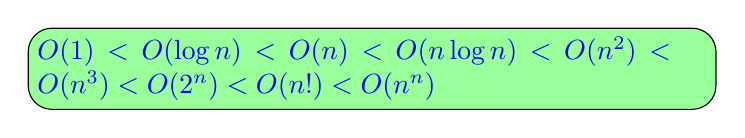
\begin{tikzpicture}
      \node [fill=green!40,draw,rectangle,rounded corners=3mm,text width=8.5cm,text=blue]
      (2) {
        $O(1)<O(\log n)<O(n)<O(n\log n)<O(n^2)<O(n^3)<O(2^n)<O(n!)<O(n^n)$
      };
    \end{tikzpicture}        
  \end{figure}
\end{frame}


\begin{frame}
  \begin{figure}
  \centering
  \begin{tikzpicture}[node distance=4cm]
    \node [fill=blue!20,draw,starburst,drop shadow,text width=2cm,text=blue] (1) {
      {\large 最坏情况}
    };
    \node [below left of=1,fill=red!20,draw,rectangle,rounded corners=4mm,text width=5.5cm] (2) {
      在$n$维随机数组中查找某个数字,
      \begin{itemize}
      \item 最好情况是出现在第一个位置,时间复杂度为$O(1)$;
      \item 最坏情况是出现在最后一个位置,时间复杂度为$O(n)$.
      \end{itemize}
    };

    \pause 
    \node at (3,-5)[text width=4.5cm,decorate,decoration=saw,fill=blue!20,draw,circle]{
      最坏情况运行时间是一种保证,亦即运行时间将不会再坏了。在应用中,这是一种最重要的需求,通常,除非特别指定,我们提到的运行时间都是最坏情况的运行时间。
    };
  \end{tikzpicture}
  
\end{figure}

\end{frame}

\begin{frame}
  \begin{figure}
  \centering
  \begin{tikzpicture}[node distance=4cm]
    \node [fill=blue!20,draw,starburst,drop shadow,text width=2cm,text=blue] (1) {
      {\large 平均情况}
    };
    \node [below left of=1,fill=red!20,draw,rectangle,rounded corners=4mm,text width=5.5cm] (2) {
      在$n$维随机数组中查找某个数字,
      \begin{itemize}
      \item 从概率角度讲,该数字在每个位置的可能性相同,故平均查找时间为$n/2$。
      \end{itemize}
    };

    \pause 
    \node at (3,-5)[text width=4.5cm,decorate,decoration=saw,fill=blue!20,draw,circle]{
      平均运行时间是所有情况中最有意义的,因为它是期望的运行时间。
    };
  \end{tikzpicture}
  
\end{figure}

\end{frame}

\begin{frame}
  \begin{figure}
  \centering
  \begin{tikzpicture}[node distance=3cm]
    \node [fill=blue!20,draw,starburst,drop shadow,text width=1cm,text=blue] (1) {
      {\large 小结}
    };
    \node [below of=1,fill=red!20,draw,rectangle,rounded corners=4mm,text width=9cm] (2) {
      对算法的分析,
      \begin{itemize}
      \item 一种方法是计算所有情况的平均值,这种时间复杂度的计算方法称为\blue{平均时间复杂度};
      \item 另一种是计算最坏情况下的时间复杂度,这种方法称为\blue{最坏时间复杂度}。
      \end{itemize}
      在没有特别说明的情况下,都指最坏时间复杂度。
    };

  \end{tikzpicture}
  
\end{figure}


\end{frame}

\begin{frame}
  \begin{figure}
  \centering
  \begin{tikzpicture}[node distance=4cm]
    \node [fill=blue!20,draw,starburst,drop shadow,text width=3.5cm,text=blue] (1) {
      {\large 算法空间复杂度}
    };
    \node [below of=1,fill=red!20,draw,rectangle,rounded corners=4mm,text width=7.8cm] (2) {
      通过计算算法所需的存储空间实现,其计算公式记作
      $$
      S(n)=O(f(n)).
      $$
      其中$n$为问题的规模,$f(n)$是语句关于$n$所占存储空间的函数。
    };
  \end{tikzpicture}
  
\end{figure}

\end{frame}

\begin{frame}
  \begin{figure}
  \centering
  \begin{tikzpicture}[node distance=0.8cm]
    \node at(0,0) [fill=blue!20,draw,starburst,drop shadow,text width=2cm,text=blue,text centered] (1) {
      {\large 总结回顾}
    };
    \pause 
    \node at(0,-1.5) [fill=red!20,draw,rectangle,rounded corners=2mm,text width=10cm,text centered] (2) {
      数据
    };
    \pause 
    \node [below of=2,fill=red!20,draw,rectangle,rounded corners=2mm,text width=10cm,text centered] (3) {
      数据对象
    };
    \pause 
    \node [below of=3,fill=red!20,draw,rectangle split,rectangle split parts=4,rectangle split horizontal,
      rounded corners=2mm,text width=2.3cm,text centered] (4) {
      数据元素 \nodepart{two}
      数据元素 \nodepart{three}
      数据元素 \nodepart{four}
      数据元素 
    };
    \pause 
    \node [below of=4,fill=red!20,draw,rectangle split,rectangle split parts=8,rectangle split horizontal,
      rounded corners=2mm,text width=1cm,text centered] (4) {
      \scriptsize{数据项1} \nodepart{two}
      \scriptsize{数据项2} \nodepart{three}
      \scriptsize{数据项1} \nodepart{four}
      \scriptsize{数据项2} \nodepart{five}
      \scriptsize{数据项1} \nodepart{six}
      \scriptsize{数据项2} \nodepart{seven}
      \scriptsize{数据项1} \nodepart{eight}
      \scriptsize{数据项2} 
    }; \pause 
    \node at (0,-6) [fill=green!40,draw,ellipse,rounded corners=2mm,text width=6cm,text centered]{
      数据结构是相互之间存在一种或多种特定关系的数据元素的集合。
    };

  \end{tikzpicture}
  
\end{figure}




\end{frame}

\begin{frame}
  \begin{figure}
  \centering
  \begin{tikzpicture}[node distance=4cm]
    \node at(0,0) [fill=blue!20,draw,starburst,drop shadow,text width=2cm,text=blue,text centered] (1) {
      {\large 总结回顾}
    };
    \pause     
    \node[below left of=1,fill=green!20,draw,rectangle split,rectangle split parts=5,rounded corners=2mm,text width=4cm,text centered,text=blue] (2) {
      \red{逻辑结构} \nodepart{two}
      集合结构 \nodepart{three}
      线性结构 \nodepart{four}
      树形结构 \nodepart{five}
      图形结构 
    };
    \pause 
    \node[below right of=1,fill=green!20,draw,rectangle split,rectangle split parts=3,rounded corners=2mm,text width=4cm,text centered,text=blue] (2) {
      \red{物理结构} \nodepart{two}
      顺序存储结构 \nodepart{three}
      链式存储结构 
    };
  \end{tikzpicture}
  
\end{figure}




\end{frame}

\begin{frame}
  \begin{figure}
  \centering
  \begin{tikzpicture}[node distance=2cm]
    \node at(0,0) [fill=blue!20,draw,starburst,drop shadow,text width=2cm,text=blue,text centered] (1) {
      {\large 总结回顾}
    };
    \pause     
    \node[below of=1,fill=green!20,draw,ellipse,text width=7.5cm,text=blue] (2) {
      \red{算法定义}:解决特定问题求解步骤的描述,在计算机中为指令的有限序列,且每条指令表示一个或多个操作。
    };
    \pause 
    \node[below of=2,fill=green!20,draw,ellipse,text width=7.5cm,text=blue] (3) {
      \red{算法特性}:有穷性、确定性、可行性、输入、输出
    };
    \pause 
    \node[below of=3,fill=green!20,draw,ellipse,text width=7.5cm,text=blue] (4) {
      \red{算法设计要求}:正确性、可读性、健壮性、高效率和低存储。
    };
  \end{tikzpicture}
  
\end{figure}




\end{frame}

\begin{frame}
  \begin{figure}
  \centering
  \begin{tikzpicture}[node distance=3cm]
    \node at(0,0) [fill=blue!20,draw,starburst,drop shadow,text width=2cm,text=blue,text centered] (1) {
      {\large 总结回顾}
    };
    \pause     
    \node[below of=1,fill=green!20,draw,ellipse,text width=7.5cm,text=blue] (2) {
      \red{算法度量方法}:事后统计方法(不科学、不准确)、事前分析估算方法。
    };
    \pause 
    \node[below of=2,fill=green!20,draw,ellipse,text width=7.5cm,text=blue] (3) {
      \red{函数的渐近增长}:  给定两个函数$f(n)$和$g(n)$,若$\exists N \in \mathbb N$, s.t. $\forall n>N$, $f(n)$总是比$g(n)$大,
      我们就说$f(n)$的增长渐近快于$g(n)$.
    };
  \end{tikzpicture}
  
\end{figure}




\end{frame}

\begin{frame}
  \begin{figure}
  \centering
  \begin{tikzpicture}[node distance=4cm]
    \node at(0,0) [fill=blue!20,draw,starburst,drop shadow,text width=2cm,text=blue,text centered] (1) {
      {\large 总结回顾}
    };
    \pause     
    \node[below of=1,fill=green!20,draw,ellipse,text width=8cm,text=blue] (3) {
      \red{大$O$阶推导过程}\\
      \begin{enumerate}[(1)]
      \item 用常数1取代运行次数中的所有加法常数;
      \item 在修改后的运行次数函数中,只保留最高阶项;
      \item 如果最高阶项存在且不是1,则去除最高阶项的系数。
      \end{enumerate}
      得到的结果就是大O阶。
    };
  \end{tikzpicture}
  
\end{figure}




\end{frame}


\begin{frame}
  \begin{figure}
  \centering
  \begin{tikzpicture}[node distance=2cm]
    \node at(0,0) [fill=blue!20,draw,starburst,drop shadow,text width=2cm,text=blue,text centered] (1) {
      {\large 总结回顾}
    };

    \pause 
    \node[below of=1,fill=green!20,draw,ellipse,text width=8cm,text=blue] (2) {
      $O(1)<O(\log n)<O(n)<O(n\log n)<O(n^2)<O(n^3)<O(2^n)<O(n!)<O(n^n)$
    };
    \pause 
    \node[below of=2,fill=green!20,draw,ellipse,text width=8cm,text=blue] (3) {
      算法最坏情况和平均情况,以及空间复杂度的概念。
    };

  \end{tikzpicture}
  
\end{figure}




\end{frame}


